\chapter{Results: Spectroscopy}

The spectroscopy of Ba in SXe was studied in detail beyond that reported in \cite{Shon,Brian}, with the goal of imaging single Ba atoms.  Emission and excitation spectra are analyzed in \ref{sec:fluorescence}, with particular interest in the origin of the 619-nm peak in \ref{sec:619identification}.  Studies of temperature and bleaching effects in \ref{sec:tempanneal} and \ref{sec:bleaching} aid in determining optimal conditions for observation.  Finally, candidate emission lines for Ba\textsuperscript{+} in SXe are discussed in \ref{sec:BaPlus}.

%Backgrounds are analyzed in \ref{sec:bgs} in order to optimize sensitivity,

\section{Excitation and Emission of Ba in SXe}
\label{sec:fluorescence}

Deposits of Ba in SXe absorb primarily between 540~nm and 570~nm.  An absorption spectrum, obtained by observing absorption of white light by a large Ba deposit at 10~K, is shown in Fig. \ref{fig:BaAbs}.  Significant broadening, as well as a 4-nm redshift  of the central peak, occur relative to the vacuum $6s^{2}$ $^{1}$S$_{0} \rightarrow 6s6p$ $^{1}$P$_{1}$ absorption value of 553.5~nm.  Initial discovery of this absorption and emission was done with the neutral Ba getter source \cite{Mong2015,Shon,Brian}.  The emission spectrum in Fig. \ref{fig:BaAbs} was obtained by 557-nm excitation of a Ba\textsuperscript{+} deposit, made at 45~K and observed at 11~K.  Observation of the same 577- and 591-nm fluorescence peaks from Ba getter deposits demonstrates that these peaks are emission of neutral Ba, and also demonstrates some neutralization of the ions \cite{Mong2015,Shon,Brian}.  The fraction of ions neutralized has not been determined.

\begin{figure} %[H]
        \centering
                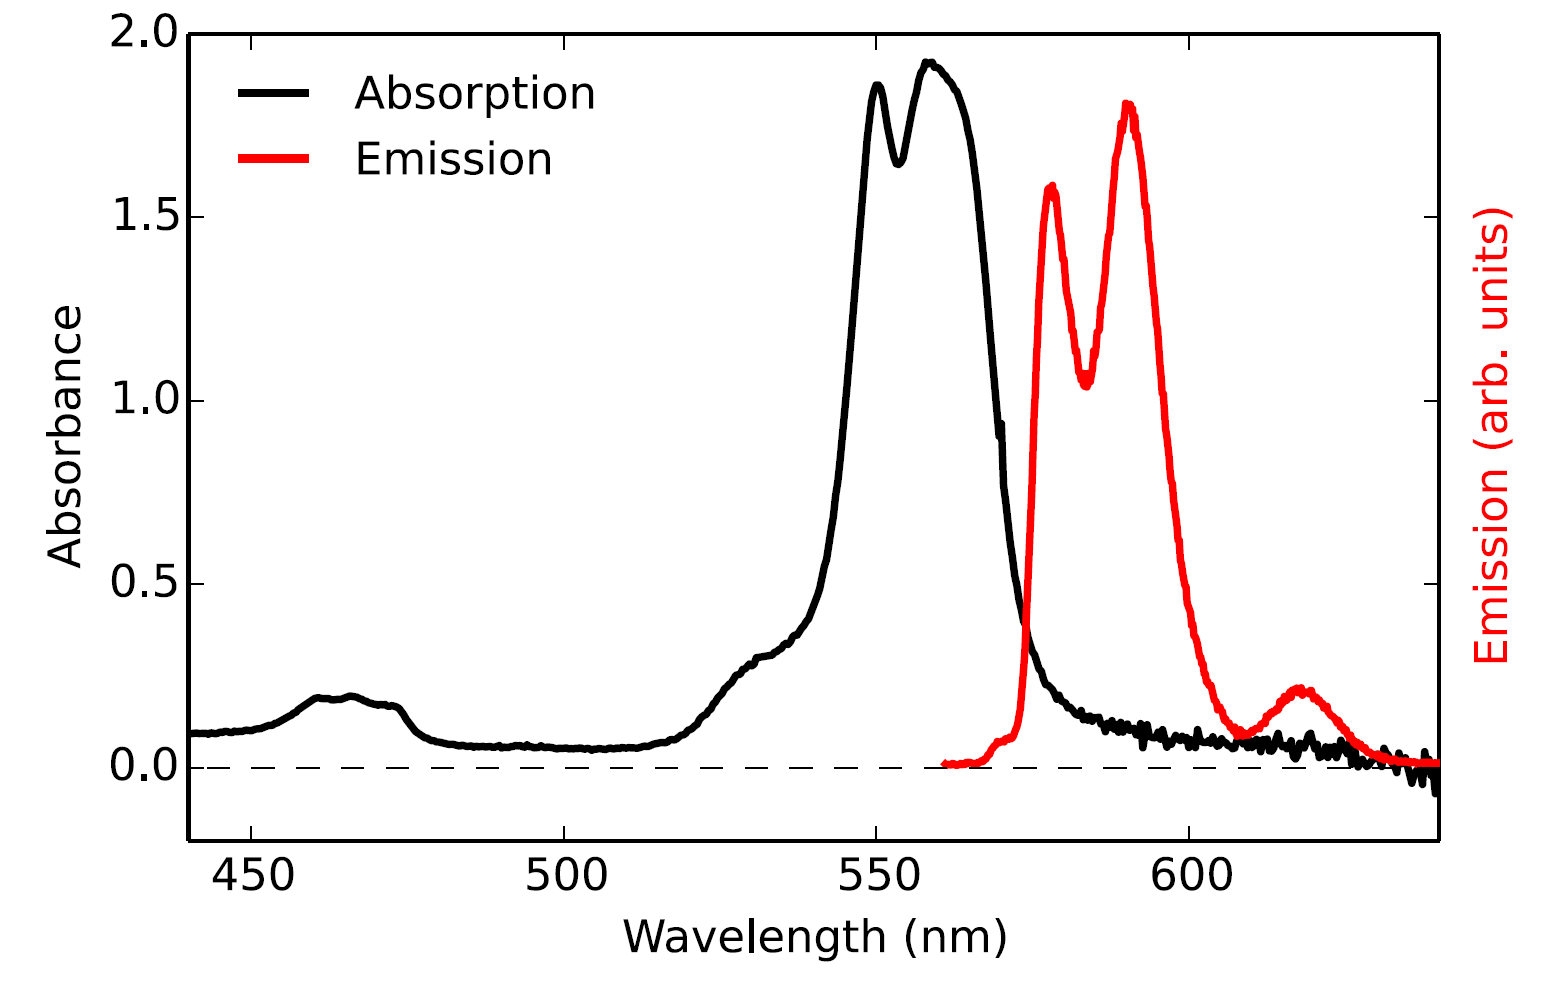
\includegraphics[width=.7\textwidth]{figures/BaAbs_fromBaSpec.png}
                \caption{Absorption and emission spectra of neutral Ba in SXe.  The absorption is of a Ba getter deposit at 10~K, and the emission is of a (neutralized) Ba\textsuperscript{+} deposit, deposited at 45~K and observed at 11~K with 557~nm excitation.\cite{Mong2015}}
\label{fig:BaAbs}
\end{figure}

\begin{figure} %[H]
        \centering
                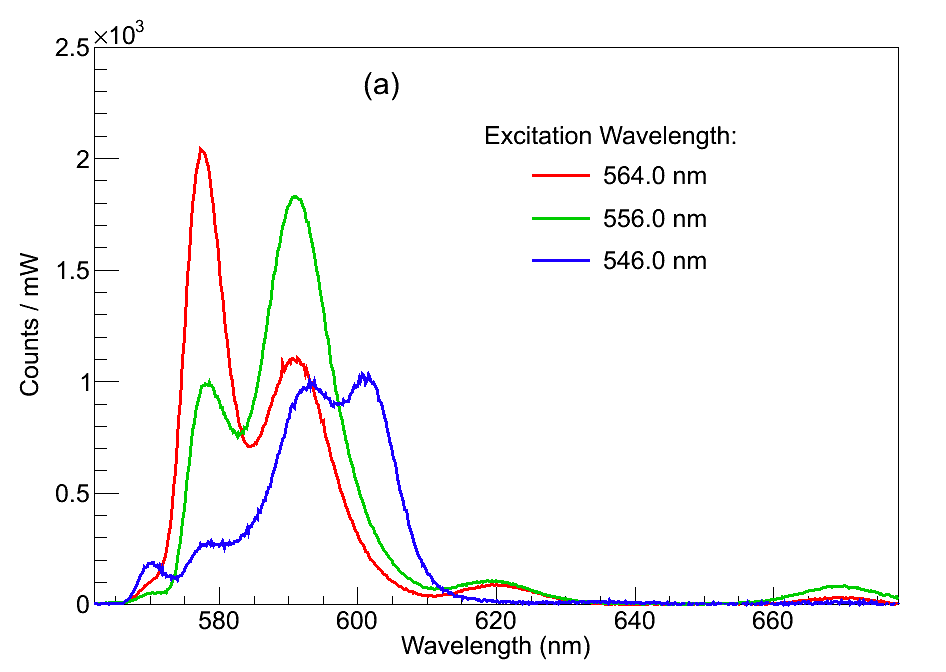
\includegraphics[width=.8\textwidth]{figures/excitspec_grn_spectra_v3.png}
                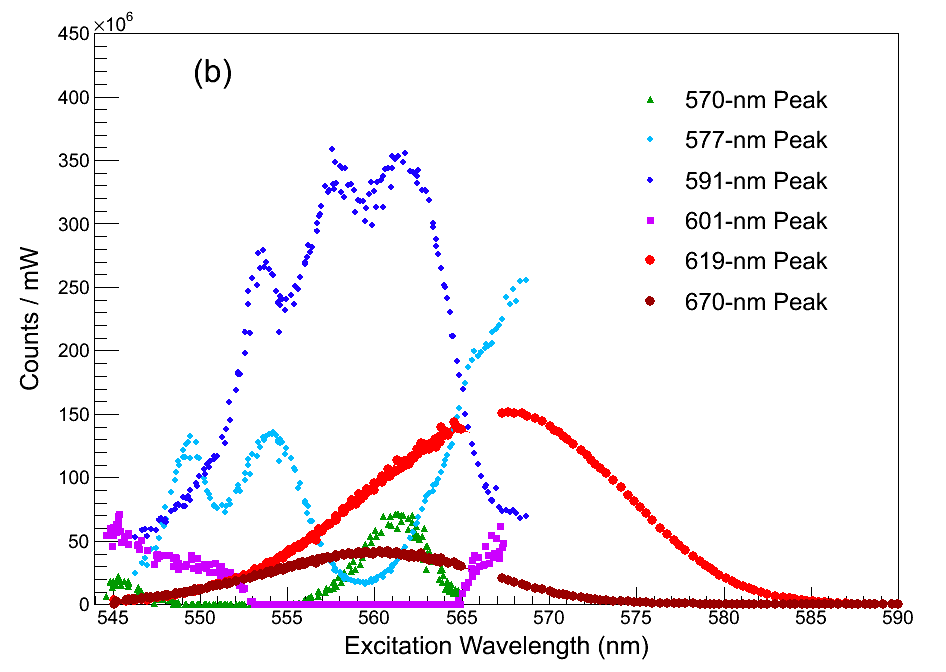
\includegraphics[width=.8\textwidth]{figures/excitspec_grn.png}
                \caption{(a) Background-subtracted fluorescence spectra for a few different excitation wavelengths, and (b) excitation spectra for all observed Ba fluorescence peaks.  Magnitudes in (b) have been scaled for visibility on the same plot.  Exposures are 1~s.}
\label{fig:excitspecGrn}
\end{figure}

%(relative magnitudes are arbitrary as they are affected by relative site populations and fluorescence efficiencies)

%Put legend in (b)? It's crowded.

%\begin{equation}
%A(1+erf(\frac{x-a}{\sigma_{1}})(1-erf(\frac{x-a}{\sigma_{2}}))
%\label{eqn:specfit}
%\end{equation}

Deposition at temperatures higher than 10~K and exploration of more excitation wavelengths have led to discovery of emission peaks beyond the 591- and 577-nm peaks reported in \cite{Shon} and \cite{Brian}.  Emission spectra for selected excitation wavelengths are shown in Fig. \ref{fig:excitspecGrn}(a) for a deposit made at 44~K and observed at 11~K.  

Excitation spectra, shown in Fig. \ref{fig:excitspecGrn}(b), were produced by scanning the dye laser and measuring the magnitude of each fluorescence peak vs. excitation wavelength.  For each frame, the spectrum was fit with a sum of peak-specific fit functions, where function shape parameters were fixed (centers and widths) and magnitudes were allowed to float.  Fitting is described in Section \ref{sec:fitting}.  The discontinuity around 566~nm for the 619- and 670-nm peaks is the boundary between the scan range of different laser dyes.  R6G dye was used for higher wavelengths and R110 for lower wavelengths.  Curves were scaled for visibility on the same plot.  Excitation was done using laser waists (w) of (1) w = 7~mm for the 570-, 577-, 591-, and 601-nm peaks, (2) w = 1000~$\mu$m for the 619- and 670-nm peaks in the R110 range, and (3) w = 200~$\mu$m for the 619- and 670-nm peaks in the R6G range.  Due to these different laser waists, as well as different deposit sizes, curves for the R6G segments (619- and 670-nm peaks) required special scaling to line up with their respective R110 segments.  This scaling was slightly different between the 619- and 670-nm peaks, likely due to different relative populations of those sites on the different deposits.

%INFO:  619- and 670-nm deposits had 5 s DC, with 24 nA on R110 one and 41.5 nA on R6G one

\section{619-nm Peak Identification}
\label{sec:619identification}

\begin{figure} %[H]
        \centering
                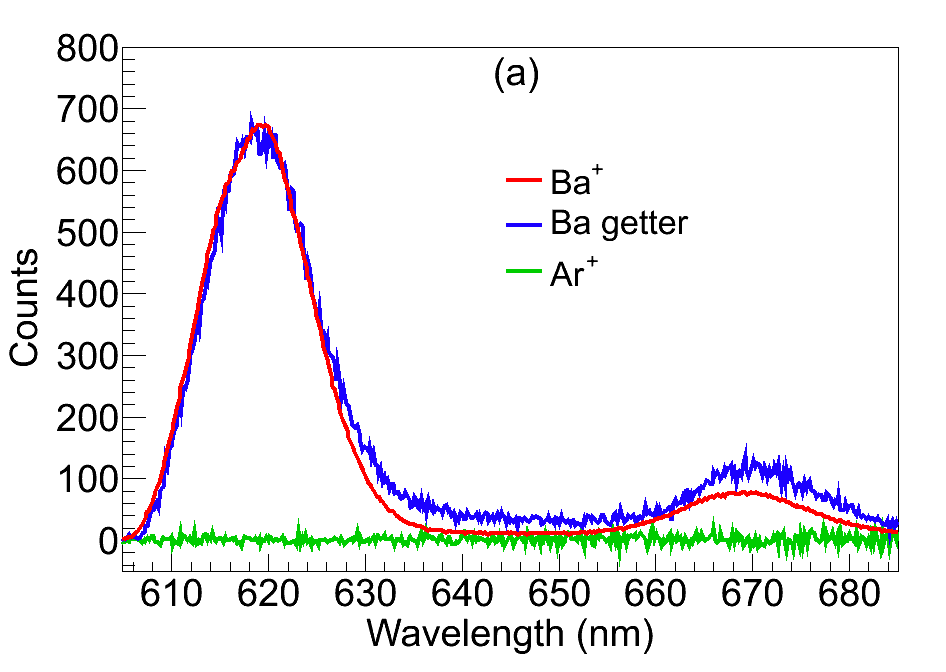
\includegraphics[width=.5\textwidth]{figures/Ar_vs_Ba.png}
                ~
                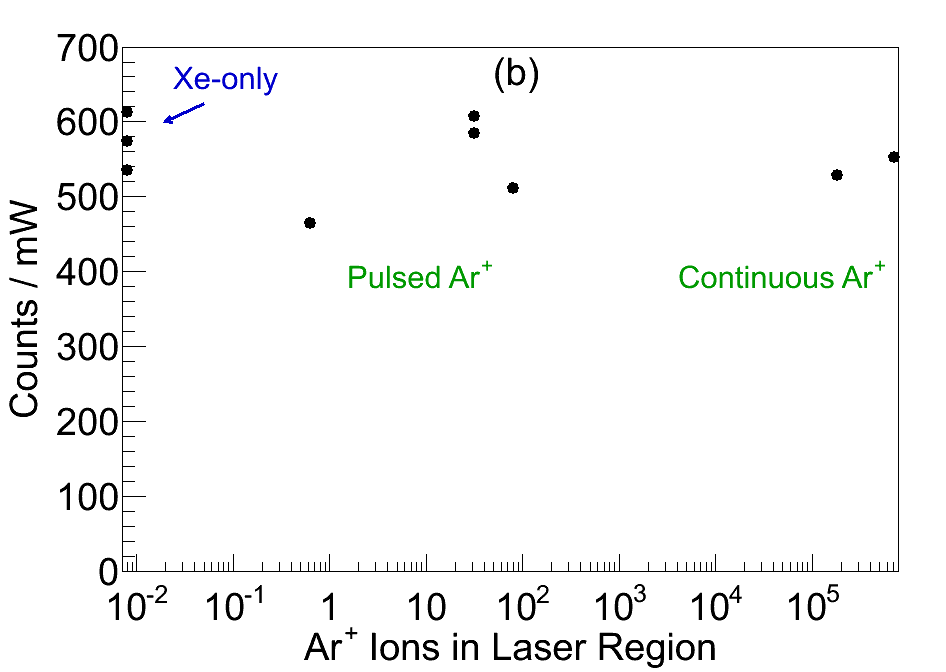
\includegraphics[width=.5\textwidth]{figures/ArImaging.png}
                \caption{Comparison of signal observed for deposits with the Ba\textsuperscript{+} ion beam (red), Ba getter (blue), and Ar\textsuperscript{+} ion beam (green) (a), and signal through 620-nm band-pass from deposits of small to large numbers of Ar\textsuperscript{+} ions in SXe.}
\label{fig:ArVsBa}
\end{figure}

The 619-nm peak, as well as the 670-nm peak, was attributed to neutral Ba by a few further tests.  A large Ba\textsuperscript{+} deposit is compared to a deposit made with the Ba getter in Fig. \ref{fig:ArVsBa}(a).  The 619-nm and 670-nm peaks were observed with both sources, and since the getter produces only neutral Ba, they were attributed to neutralized ions in Ba\textsuperscript{+} deposits.  Observation of the fluorescence with two different types of Ba sources is itself positive.  In addition, observation of the fluorescence with the low deposit energy of the getter may bode well for the prospect of grabbing on a probe in LXe.  Observation of a large deposit of Ar\textsuperscript{+} in SXe is also shown in Fig. \ref{fig:ArVsBa}(a).  The lack of fluorescence further disfavors a matrix-damage-related source of the fluorescence, such as color centers.  Finally, to rule out the possibility that the signal in Ba imaging experiments is due to passed wavelengths far from the 620-nm band-pass region, e.g. infrared, imaging experiments of Ar\textsuperscript{+} deposits in SXe were performed with both pulsing and continuous ion beams.  The same 620-nm band-pass filter was used, as well as the same focused 570-nm laser, to be similar to Ba\textsuperscript{+} 619-nm imaging experiments.  Summed counts from these deposits were consistent with background, as shown in Fig. \ref{fig:ArVsBa}(b).

%at one point youthought leak rate dependence could go here

\section{Annealing/Temperature Dependence}
\label{sec:tempanneal}

%\emph{\color{gray}When does it need to be mentioned that certain data was also used in the paper(s)?}

%Matrix site occupancies for Ba atoms

\begin{figure} %[H]
        \centering
                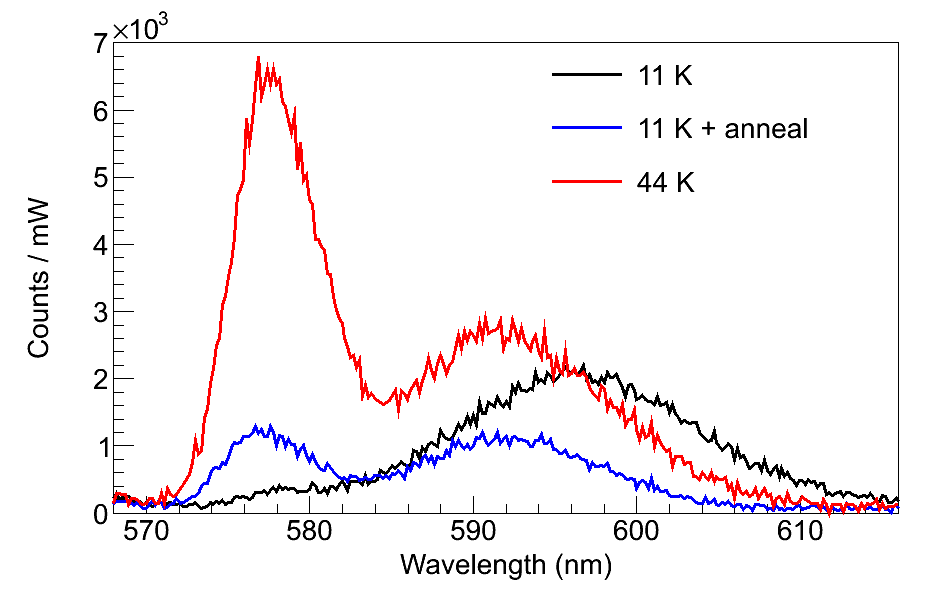
\includegraphics[width=.7\textwidth]{figures/spectra_temperature_conditions.png}
                \caption{Spectra of peaks around 590~nm of a Ba\textsuperscript{+} deposit made at 11~K before and after annealing to 39.4~K, and one made at 44~K.  All observations are at 11~K.  Both Ba\textsuperscript{+} deposits are 15~s, however the 44~K deposit is scaled slightly to account for different ion current.  Laser power was about 0.1~mW with an unfocused beam waist of w = 7.056~mm, at 566~nm wavelength.}
\label{fig:specTempConditions}
\end{figure}

\begin{figure} [h]
        \centering
                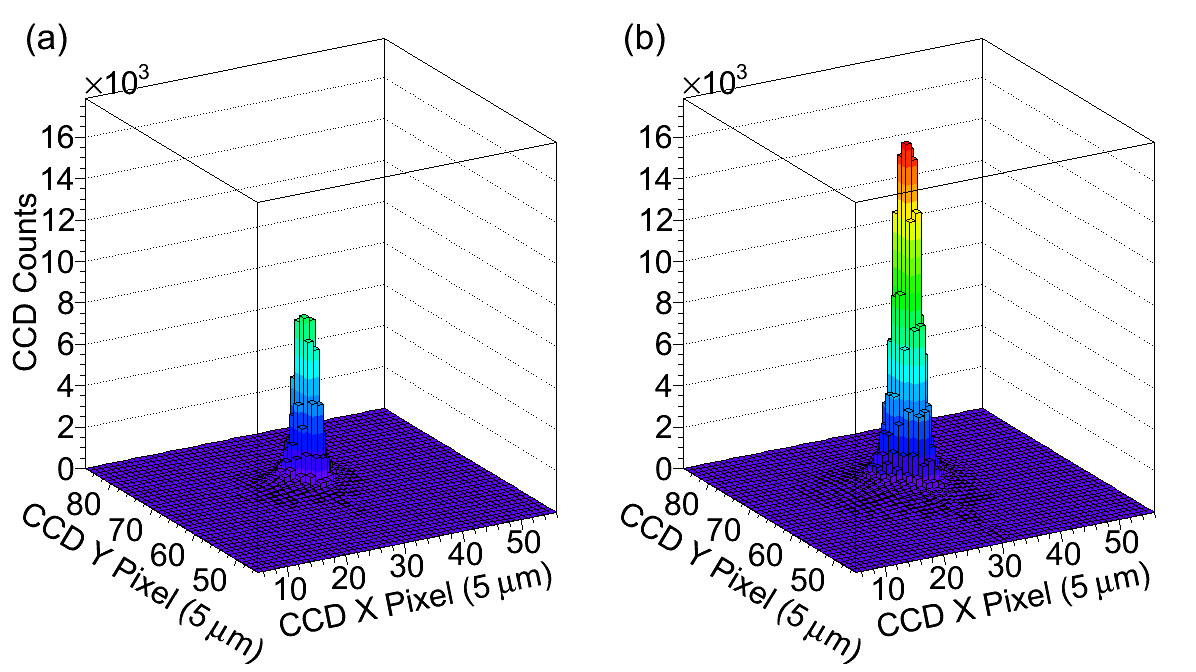
\includegraphics[width=.8\textwidth]{figures/619_deposit_temp.png}
                \caption{Images of 619-nm fluorescence in focused 570-nm laser region for deposits made at (a) 11K and (b) 52~K.  Deposits are 3~s of continuous Ba\textsuperscript{+} current.  Exposures are 0.1~s at 11~K.}
\label{fig:specTempConditions619}
\end{figure}

Emission spectra can depend on annealing history, and similarly on the temperature at which a deposit is made.  Spectra under different temperature conditions are shown in Fig. \ref{fig:specTempConditions}.  Peak shapes look similar for deposits made at 40-55~K to those made at 11~K and then annealed to 40-55~K, where both are observed at 11~K.  Differences in relative amplitudes could be due to differences in matrix site populations.  The broader emission around 596~nm in non-annealed 11-K deposits is interpreted as a higher population of the 601-nm peak, as it is not resolved from the 591-nm peak.  Deposit temperature dependence of the 619-nm peak was studied by imaging the fluorescence from a focused laser through the 620-nm band-pass filter, shown in Fig. \ref{fig:specTempConditions619}.  The level of 619-nm signal is about 3$\times$ larger in deposits made at 52~K vs. 11~K.  Imaging is described in detail in Chapter 6.  These tests guided the standard of depositing at 50$\pm$5~K when observing the 577-, 591-, and/or 619-nm peaks.

%the respective 31~nm/s and 37~nm/s are from the same Xe leak rate, resulting in different SXe deposition rates daccording to Fig. \ref{fig:fringes_52K_vs_11K}

%A study of deposit conditions for the 619-nm peak (rather than just temp-depend)

% is discussed briefly in \ref{sec:bleaching}.

%5.4E4 Xe:Ba for leak 48 50~K (31 nm/s)

% at leak setting 48 (619 vs temp)

\begin{figure} %[H]
        \centering
                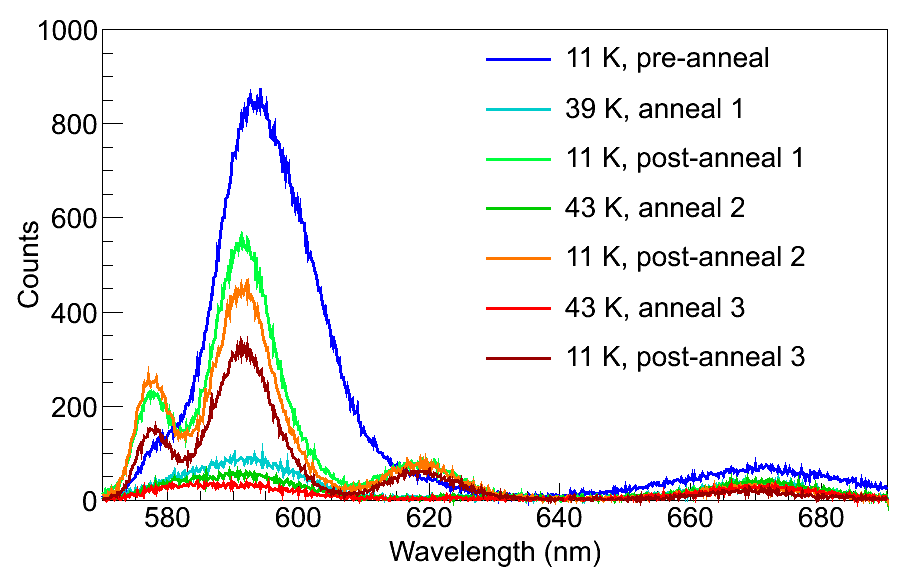
\includegraphics[width=.7\textwidth]{figures/spectra_annealing.png}
                \caption{Spectra of a large Ba\textsuperscript{+} deposit through several annealing cycles.  Initial deposit was at 11~K.  Laser power was about 0.2~mW with an unfocused beam waist of w = 7.056~mm, at 564~nm wavelength.  These are selections from the full data set shown as peak counts vs. temperature in Fig. \ref{fig:annealGrn}.  \cite{Mong2015}}
\label{fig:specAnneal}
\end{figure}

\begin{figure} %[H]
        \centering
%                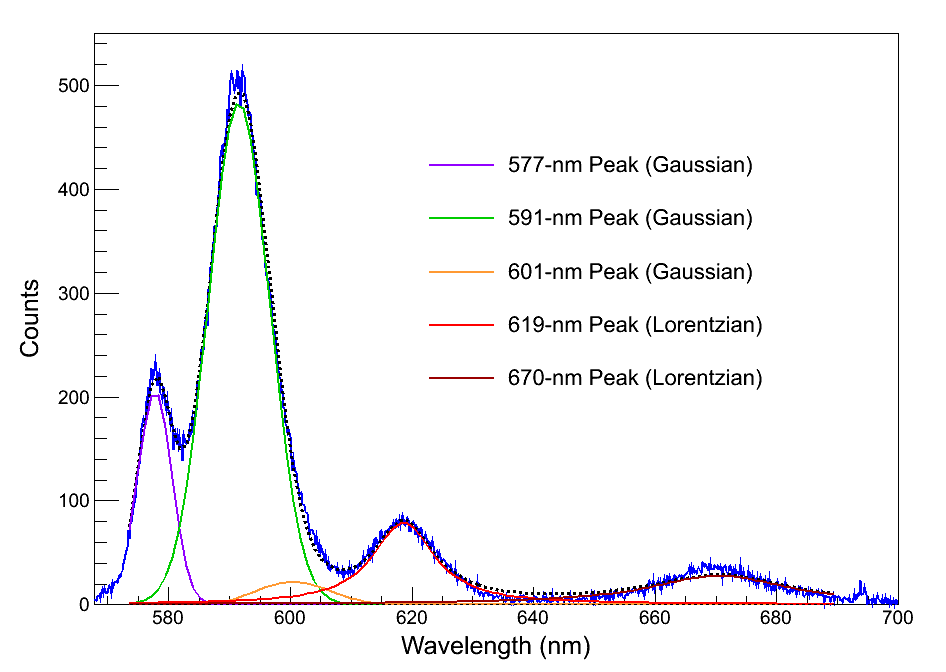
\includegraphics[width=.5\textwidth]{figures/spectra_anneal_fit.png}
%                ~
                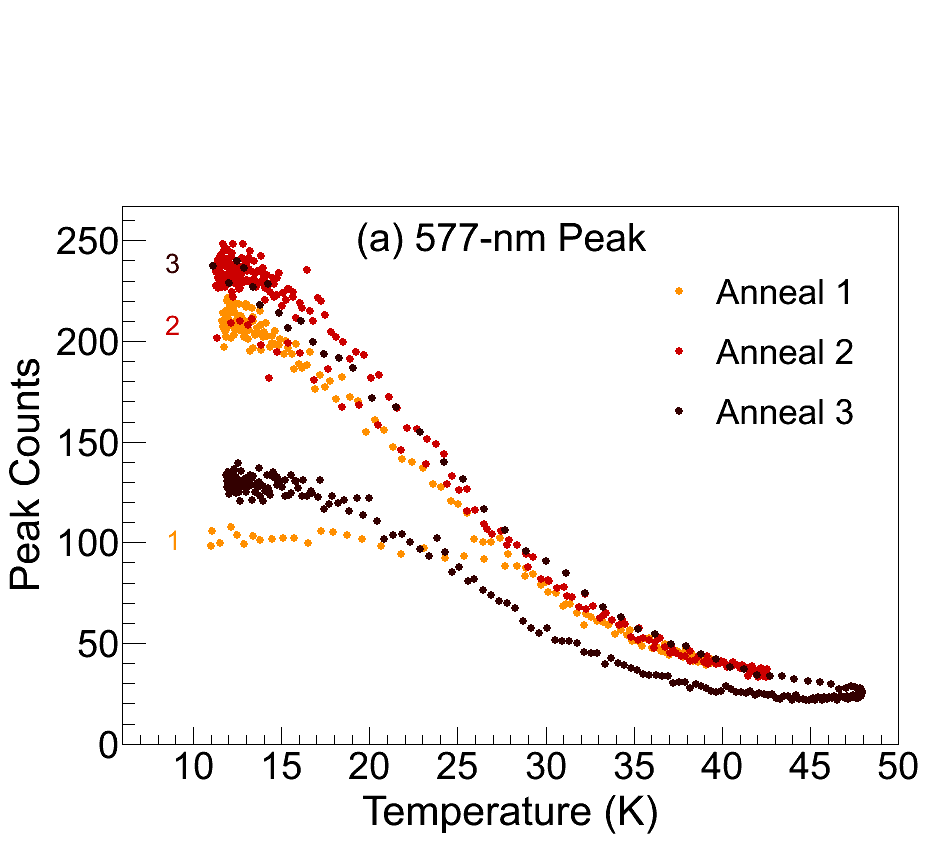
\includegraphics[width=.5\textwidth]{figures/anneal_577peak_topspace.png}
                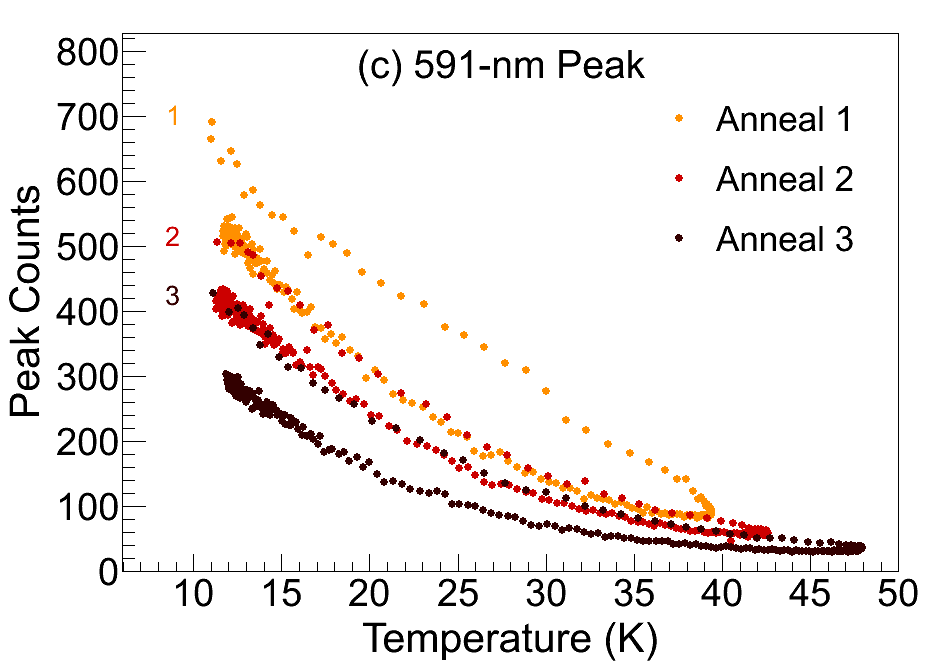
\includegraphics[width=.5\textwidth]{figures/anneal_591peak.png}
                ~
                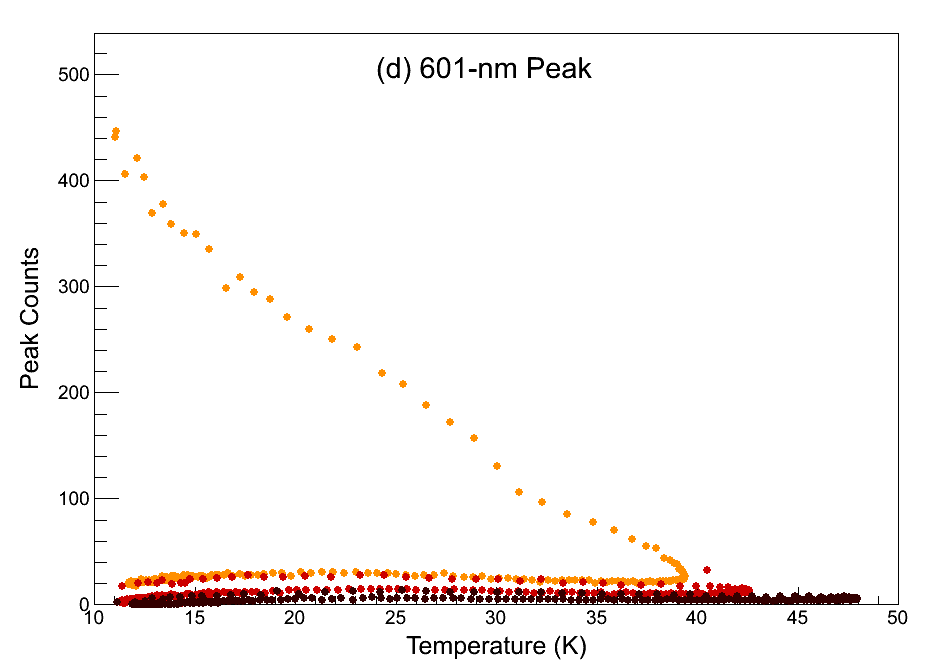
\includegraphics[width=.5\textwidth]{figures/anneal_601peak.png}
                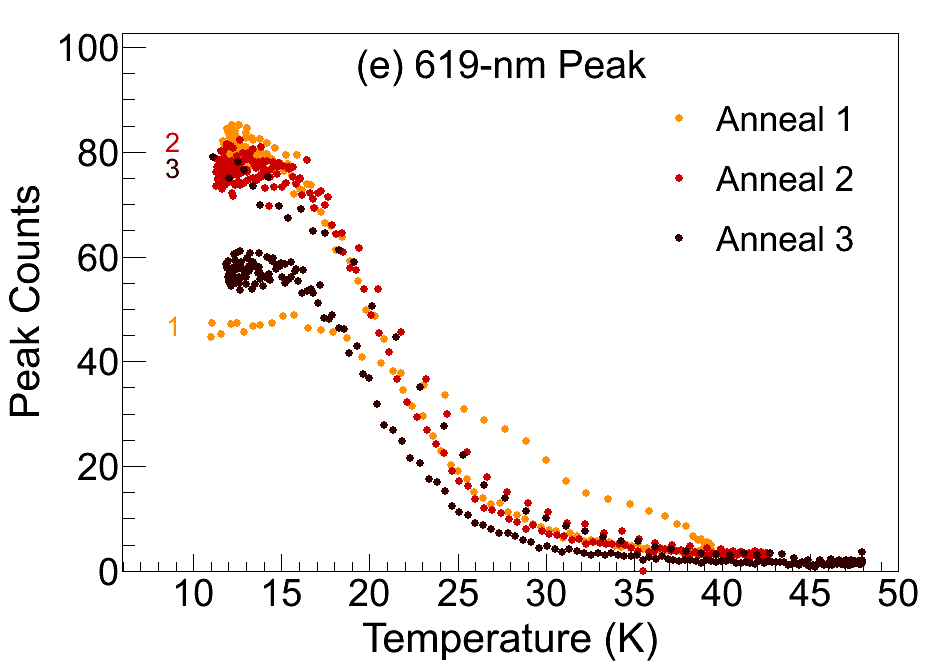
\includegraphics[width=.5\textwidth]{figures/anneal_619peak.png}
                ~
                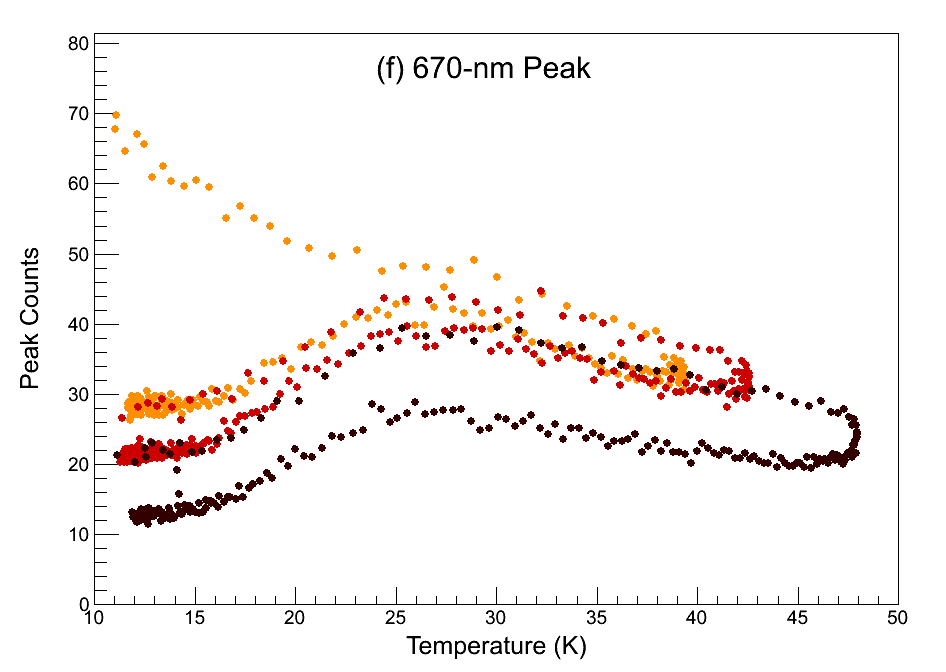
\includegraphics[width=.5\textwidth]{figures/anneal_670peak.png}
                \caption{Fit peak counts for the (a) 577-, (b) 591-, (c) 601-, (d) 619-, and (e) 670-nm fluorescence peaks through three annealing cycles of the Ba\textsuperscript{+} deposit made at 11~K.  ``1", ``2", and ``3" mark the beginning of each anneal cycle.  Laser power was about 0.2~mW with an unfocused beam waist of w = 7.056~mm, at 564~nm wavelength.}
\label{fig:annealGrn}
\end{figure}
%\clearpage weird

Fluorescence spectra with 564~nm excitation through several annealing cycles for a deposit made at 11~K are shown in Fig. \ref{fig:specAnneal}.  At this wavelength, all obserrved Ba peaks are prominent except the 570-nm peak.  Initial exposure shows significant 591- and 601-nm (unresolved from one another) emission, with some 577-nm emission.  All peaks are reduced at the high temperature ends of the anneal cycles, and return to lower temperatures shows recovery to an overall increase for some peaks, and overall loss of others.  Fit peak counts (fitting is described in Sec. \ref{sec:fitting}) vs. temperature are shown in Fig. \ref{fig:annealGrn}.  The 577-nm and 619-nm peaks gained significantly with the first anneal, suggesting that they are due to more stable matrix sites.  Both of these peaks remained about the same after the second cycle (small gain in 577-nm), and both had loss after the third cycle, which reached the higher temperature of 48~K.  The 591-nm had moderate loss with each cycle.  The 601-nm peak had nearly complete loss in the first anneal cycle.  The 670-nm peak had significant loss, with more loss after each succeeding anneal cycle, each of which reached higher a temperature than the last.

%This could be due to greater diffusion at higher temperature leading to Ba/Ba interactions.

% In this interpretation, the 601-nm peak along with the 591-nm peak fit the broader peak in the initial 11~K deposit.

Aside from matrix site changes, direct temperature dependence of fluorescence can be observed in annealing cycles.  The 577-, 591- and 619-nm peaks have their highest amplitude at 11~K.  The 577-nm and 619-nm peaks reach a plateau at 11~K, while the 591-nm may benefit from even lower temperatures.  The inverse relationship between fluorescence of these major peaks and temperature suggests that a probe in nEXO will need to be moved to an evacuated chamber in order to cool to 11~K or below for observation.  

% After annealing, the 670-nm peak has its highest amplitude at around 25~K.

%\emph{\color{gray}601 and (not shown) 570 would require different wavelength to study.}

%[inverse relationship] could be due to a different matrix environment at higher temperature, or possibly a loss of fluorescence efficiency due to increased non-radiative decays from the excited state.  

%\vspace{40mm}
\section{Bleaching}
\label{sec:bleaching}

% QUESTION: \emph{\color{gray}Just show bleaching, as informant on how to image, rather than showing model fits.}

Decay of fluorescence with laser exposure, or bleaching, was observed for all six Ba fluorescence peaks.  Examples of bleaching spectra are shown in Fig. \ref{fig:specBleach}, with excitation at (a) 556.9~nm, (b) 562.6~nm, and (c) 566.3~nm, using a semi-focused laser of waist w = 1000 $\mu$m.  Each curve is the Ba emission spectrum at different points in time.  Bleaching was rapid for the 570-, 577-, 591-, and 601-nm peaks, and much slower for the 619- and 670-nm peaks.

\begin{figure} %[H]
        \centering
                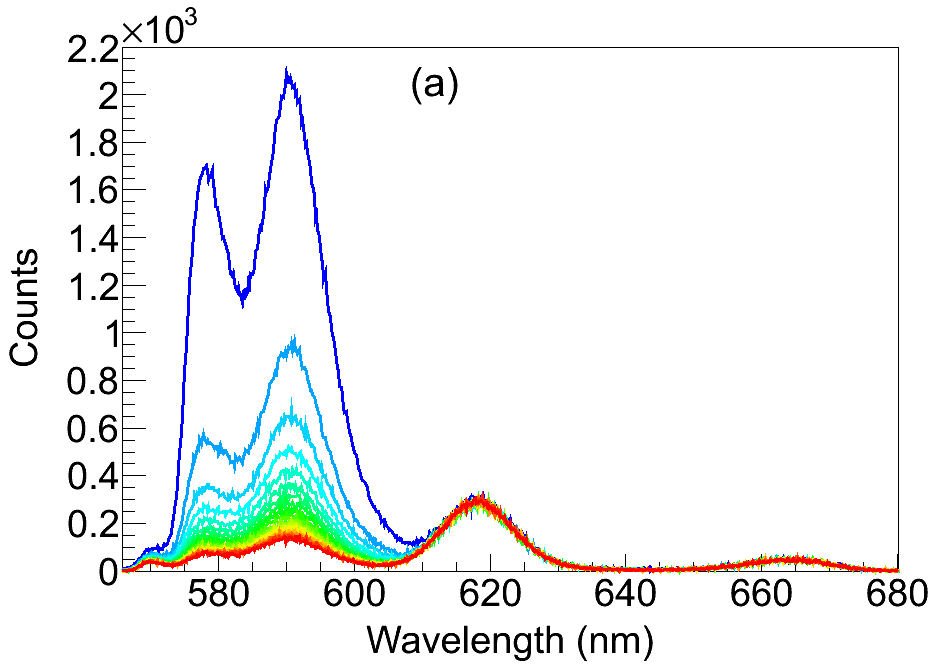
\includegraphics[width=.5\textwidth]{figures/bleach_spectra_a.png}
                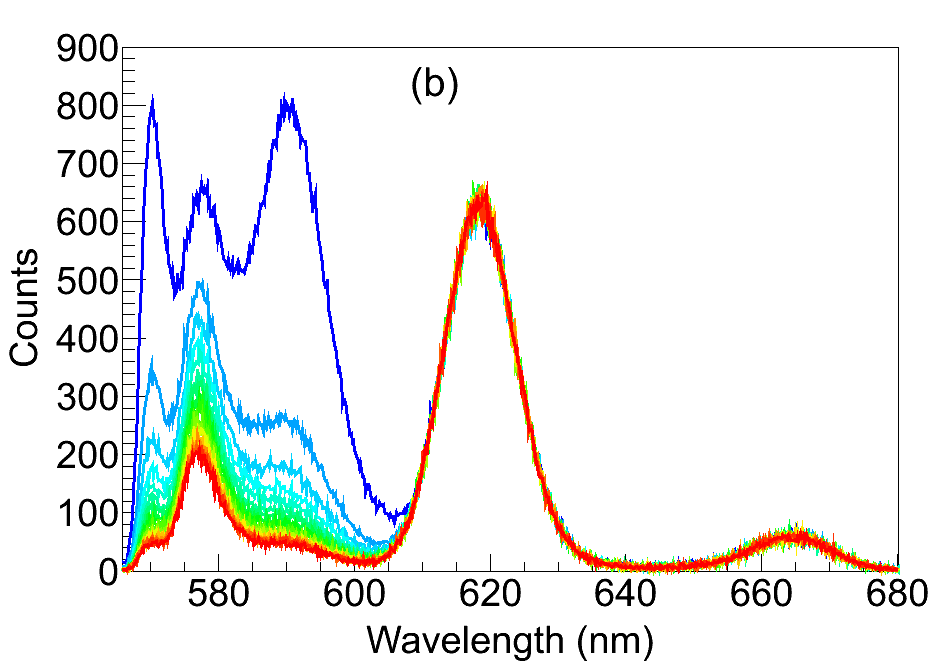
\includegraphics[width=.5\textwidth]{figures/bleach_spectra_b.png}
                ~
                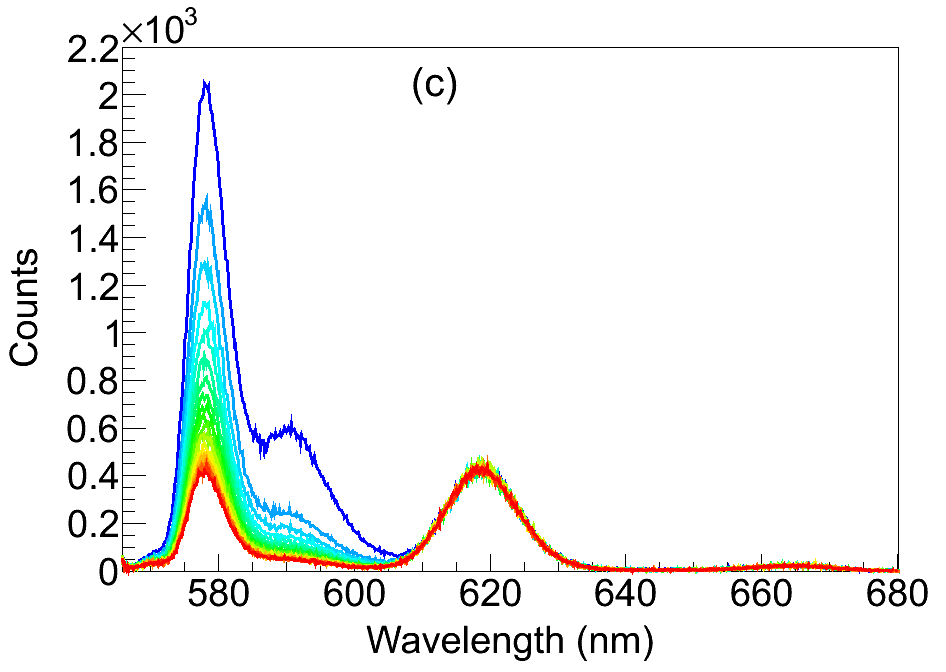
\includegraphics[width=.5\textwidth]{figures/bleach_spectra_c.png}
                \caption{Bleaching Ba emission peaks with excitation at (a) 556.9~nm, (b) 562.6~nm, and (c) 566.3~nm.  Laser power and exposure times are (a) 1.3~mW and 1~s, (b) 7.5~mW and 0.2~s, and (c) 5.8~mW and 0.2~s.  Every tenth exposure is shown, beginning with the second in the darkest blue, ending with the darkest red.  Each is a 5-s continuous Ba\textsuperscript{+} deposit at 45~K, observed at 11~K. \cite{Mong2015}}
\label{fig:specBleach}
\end{figure}

%To produce a well-known laser intensity, the laser was de-focused to a specific beam waist, and the image of 619-nm fluorescence (which defines the laser region due to its low bleaching) from a large Ba\textsuperscript{+} deposit was centered in the spectrometer slit and a y-pixel region of interest (ROI) with edges at 90\% of the maximal intensity.  Ba spectra over time are shown in Fig. \ref{fig:specBleach}(a,b,c) for excitation at (a) 556.9~nm, (b) 562.6~nm, and (c) 566.3~nm, where relative bleaching rates between peaks can be seen to depend on the excitation wavelength.

\subsection{Bleaching of the 577- and 591-nm Peaks}

\begin{figure} %[H]
        \centering
                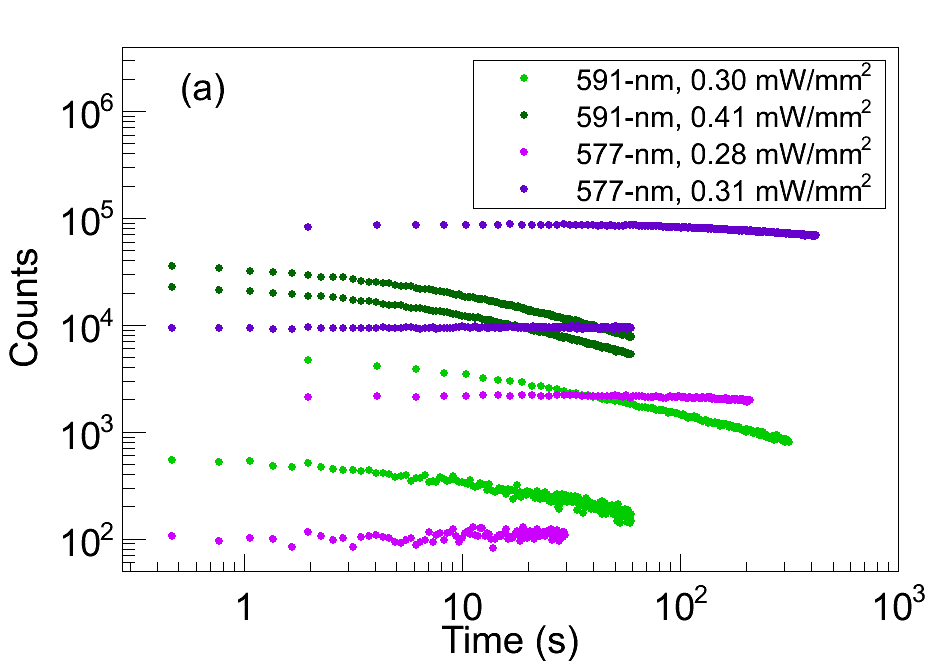
\includegraphics[width=.5\textwidth]{figures/bleach_577vs591_on-res_a_low-I.png}
                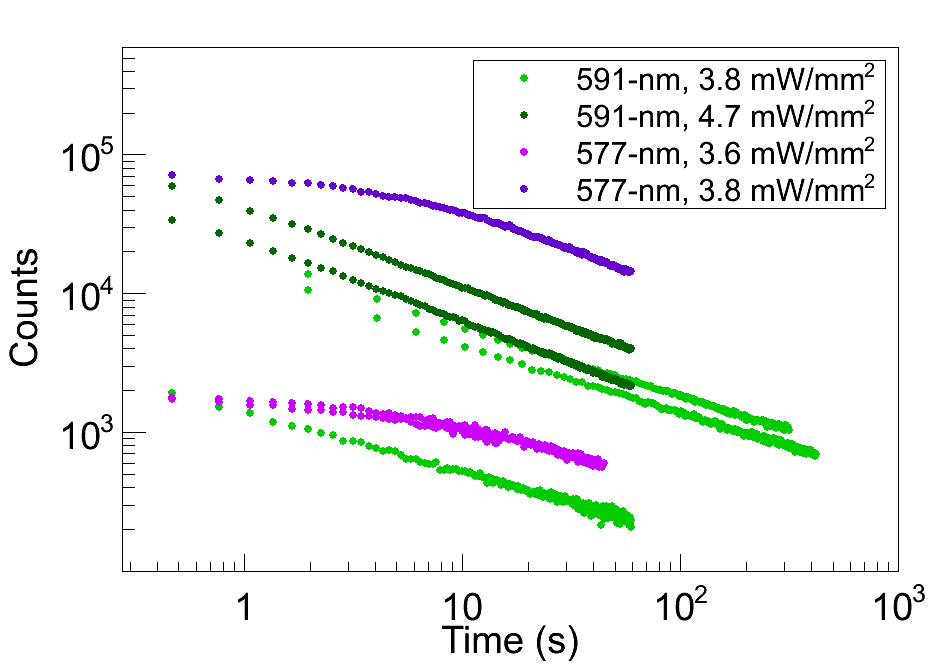
\includegraphics[width=.5\textwidth]{figures/bleach_577vs591_on-res_b_medium-I.png}
                ~
                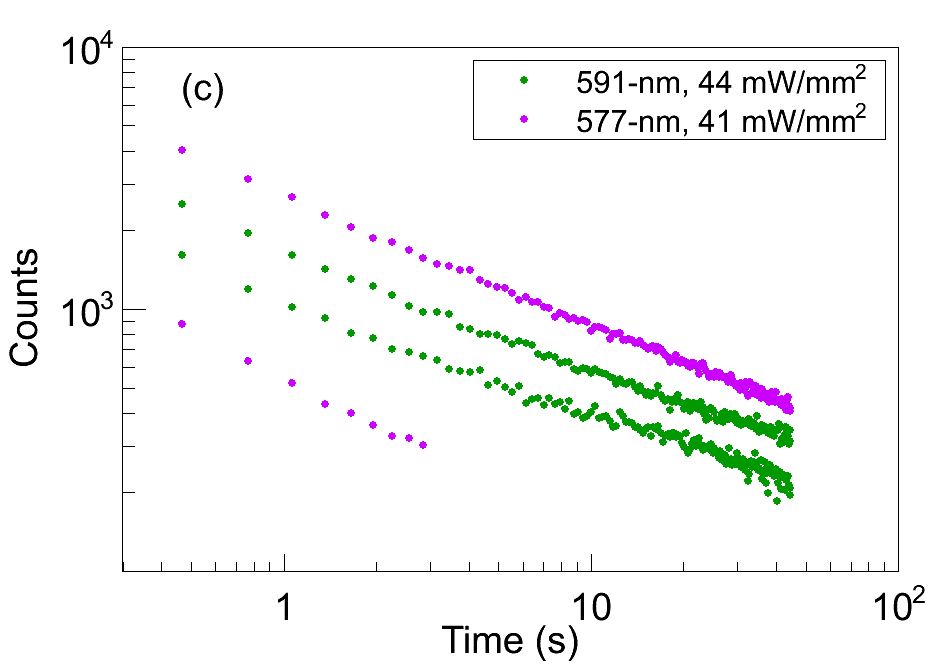
\includegraphics[width=.5\textwidth]{figures/bleach_577vs591_on-res_c_high-I.png}
                \caption{Fluorescence vs. time for three orders of magnitude (a,b,c) in laser intensity, for the 577-nm (purple) and 591-nm (green) fluorescence peaks.  Deposits are continuous Ba\textsuperscript{+} at 45~K, observed at 11~K.  Exposures are 0.2 or 2~s (indicated by point spacing minus 98.18~ms readout time).}
\label{fig:bleach_577vs591}
\end{figure}

Fit integral fluorescence counts vs. time are shows in Fig. \ref{fig:bleach_577vs591} for both the 577-nm (purple) and 591-nm (green) fluorescence peaks, with laser intensities on the order of (a) 0.33, (b) 4.0, and (c) 43 mW/mm\textsuperscript{2}.  Exact intensities are listed in the legends.  The excitation wavelengths used for these comparisons were chosen to be optimal for the respective fluorescence peak:  566.3~nm was used for the 577-nm peak, and 562.6~nm for the 591-nm peak (see Fig. \ref{fig:excitspecGrn} for excitation spectrum).  Bleaching was more rapid in the 591-nm peak when low intensity is used (a).  For medium intensity (b), bleaching was more rapid for the 591-nm peak in the first 10~s, and then began approaching a similar rate to the 577-nm peak.  For the high intensity (c), the rates began similar, with the 577-nm peak bleaching rate barely surpassing that of the 591-nm peak after about 20~s.

Comparisons of bleaching with different excitation wavelengths are shown in Fig. \ref{fig:bleach_excitCompare} for (a) the 577-nm peak, and (b) the 591-nm peak.  In the case of the 577-nm peak (a), the excitation wavelengths (566.3 and 556.9~nm) correspond to different peaks in the excitation spectrum (Fig. \ref{fig:excitspecGrn}).  Very different bleaching rates were observed (although the 556.9-nm excitation had about 2.5$\times$ the intensity).  In the case of the 591-nm peak (b), the excitation wavelengths (562.6 and 556.9~nm) correspond to neighboring peaks in the triplet structure of the excitation spectrum.  The bleaching rates are similar, with a somewhat faster rate for the 556.9-nm excitation, which had about 2$\times$ the intensity.

% as the 562.6-nm excitation

Ultimately, these studies suggested the usage of the 577-nm peak in imaging small numbers of atoms due to its lower bleaching rate, especially with excitation on the high-wavelength end of the range studied.  Imaging of Ba atoms using a combination of the 577- and 591-nm peaks with excitation at 566~nm, via a band-pass filter passing 573 - 599~nm FWHM, is discussed in Sec. \ref{sec:imaging590and577}.

\begin{figure} %[H]
        \centering
                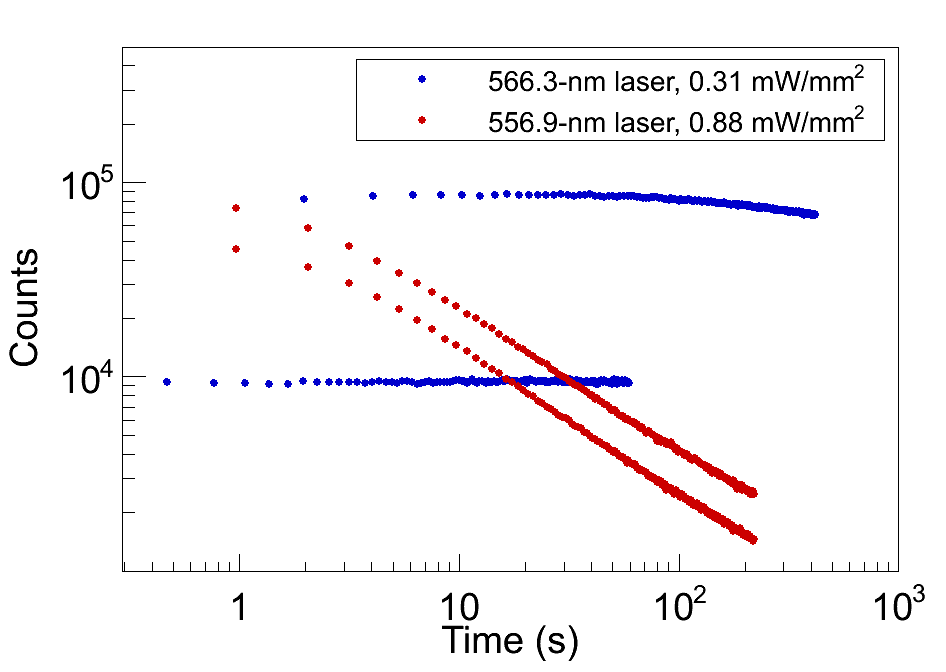
\includegraphics[width=.5\textwidth]{figures/bleach_577-nm_555vs560.png}
                ~
                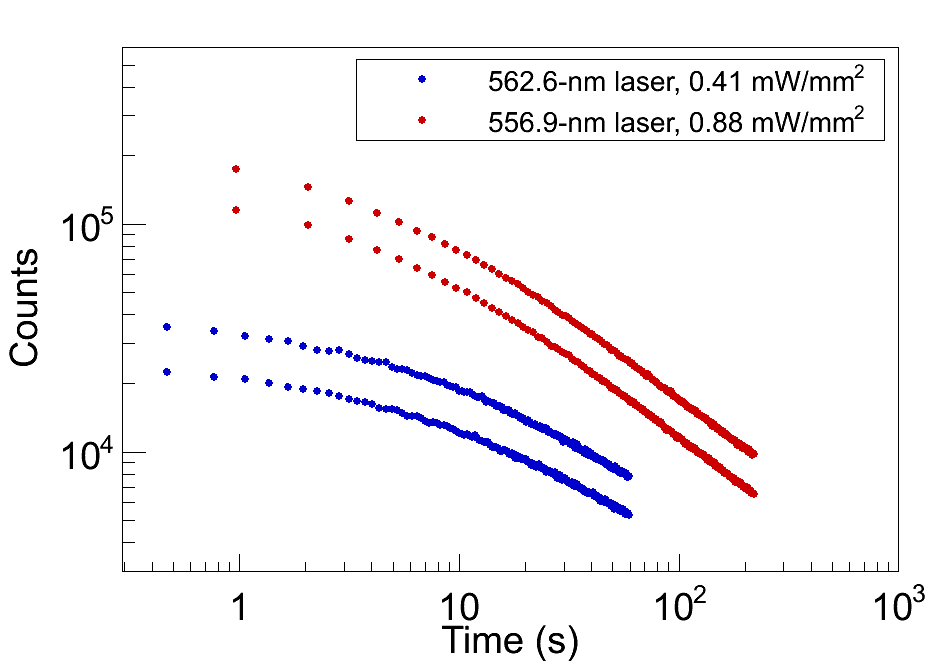
\includegraphics[width=.5\textwidth]{figures/bleach_591-nm_555vs560.png}
                \caption{}
\label{fig:bleach_excitCompare}
\end{figure}

A numerical model of fluorescence vs. time, described in Sec. \ref{sec:model} for a 5-level system of Ba in vacuum, was calculated for comparison to bleaching data.

The 6(5)-level model solved in [sec. in Ch. 2]... similar to vacuum rates is OK for beginning (fails at certain point, pretty consistent across the board) ...could draw regions A and B where there is disagreement

%talk about hole bleaching?

%\begin{figure} %[H]
 %       \centering
  %              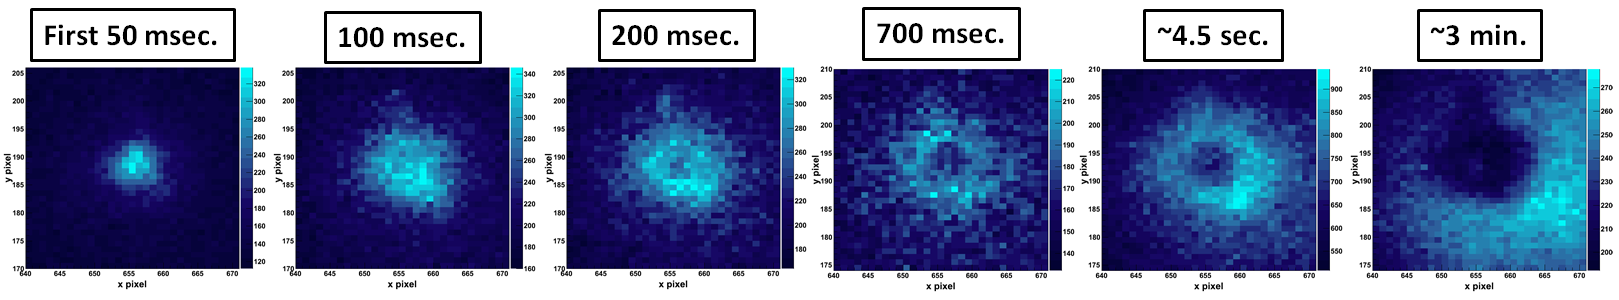
\includegraphics[width=.9\textwidth]{figures/hole_bleach_590.png}
   %             \caption{}
%\label{fig:testfig}
%\end{figure}

\subsection{Re-pumping}

%mention that similarity to vacuum rates suggests laser repumping?

Effective re-pumping of optically pumped Ba could require up to three additional lasers, one for each of the populated metastable D states, as it does in vacuum.  The optimal absorption for each transition would need to be discovered using tunable lasers in the infrared, and the search would be challenging, as the effect of re-pump is small until all three are achieved.  However, mixing of states in the Xe matrix could lower the number of lasers needed.  Searches for an effect of additional excitation lasers were attempted with a few different lasers.  A 1550-nm diode laser and a 1064-nm Nd:YAG laser were used to attempt re-pumping from the \textsuperscript{1}D and \textsuperscript{3}D states, respectively.  A 657-nm diode laser was used to attempt excitation from the \textsuperscript{3}D states into the higher-level $5d6p$ \textsuperscript{3}D$_{1}$\textsuperscript{o} state, which in vacuum has a path back to ground, as utilized in the Ba MOT in \cite{BaMOT} for the $6d5d$ \textsuperscript{3}D$_{1}$ state with 659.7~nm.  The blue C480 dye laser and 406-nm Kr ion laser were used to attempt excitation from the \textsuperscript{1}D state into the higher-level states $6s7p$ \textsuperscript{1}P$_{1}$\textsuperscript{o} and $6s8p$ \textsuperscript{1}P$_{1}$\textsuperscript{o}, respectively, which have paths back to ground in vacuum.

The only effects observed on bleaching rates by these re-pump lasers were increased bleaching by the blue dye and 406-nm Kr ion lasers.  Some effect of a return of fluorescence was observed after separate exposures of low-intensity 406-nm Kr ion laser, shown in Fig. [fig Kr return].  In this experiment, bleaching of the 591-nm peak was observed by x-nm excitation, and then the x-nm laser was blocked for a length of time, either for a waiting period or for exposure to the 406-nm laser.  Larger returns in 591-nm fluorescence were observed with 406-nm exposure than for periods of just waiting, for low intensities of the 406~nm.  However, co-exposure of this intensity of 406~nm with the green excitation laser had no noticeable effect.  This phenomenon was not explored further.

\subsection{Bleaching of the 619-nm Peak}

%Another possible mechanism for bleaching is matrix site change caused by the difference in the Ba-Xe interactions when the Ba is in the excited state.  This was explored in an experiment where excitation spectra were produced before and after bleaching the Ba sample at various wavelengths.  \emph{\color{gray}Selected} runs are shown in Fig. [bleaching excitspec].  \emph{\color{gray}describe -- interesting changes may reveal different site components of the peaks -- or does it?  idk how this could happen ... cuz the triple peak thing was supposedly normal for a single site ... small rises were ween, but poplulations cannot be known, so we don;t know}  \emph{\color{red}plots could be simple, like 2 excitspec for a single peak with an arrow at the bleaching (between) $\lambda$ w/ a note like ``bleach w/ x~mW of x~nm"...}

The 619-nm peak bleaches at much higher laser intensities.  At a few mW of around 570~nm, bleaching is observed when the laser is focused.  Integrated 619-nm fluorescence, divided by laser power, vs. time from an image of a focused 570-nm laser is shown in Fig. \ref{fig:bleaching619} for three laser powers.  Observation of lower total counts when laser intensity and exposure time are increased and decreased, respectively, by the same factor, i.e. the same number of photons on faster time scales, indicates a time-dependent return mechanism for the fluorescence.  This could be a return from a metastable state.  Alternatively, if the 619-nm bleaching is caused by laser-heating of the sample (likely by heating the sapphire window), then the time-dependent return could be defined by the cryostat cooling power.  Faster exposure times are more convenient, however this must be balanced against a loss of signal-to-noise.  The 0.21~mW laser power was chosen, corresponding to an intensity of about 11.8~$\mu$W/$\mu$m$^{2}$.

\begin{figure} %[h]
        \centering
                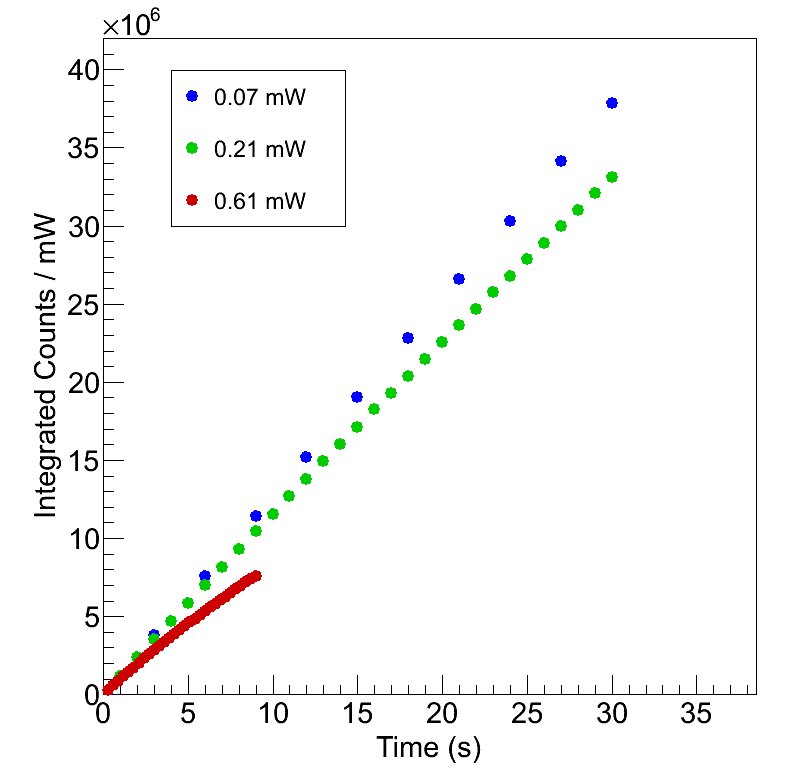
\includegraphics[width=.7\textwidth]{figures/619_bleach_summed_per_mW.png}
                \caption{}
\label{fig:bleaching619}
\end{figure}

%As indicated in Fig. \ref{fig:specTempConditions619} in \ref{sec:tempanneal}, more rapid bleaching of the 619-nm peak is observed with the lower SXe growth rate of 5~nm/s.  This is not understood, though possible explanations include 

\section{Fluorescence Efficiency of 577- and 591-nm Peaks}

\begin{figure} %[H]
        \centering
                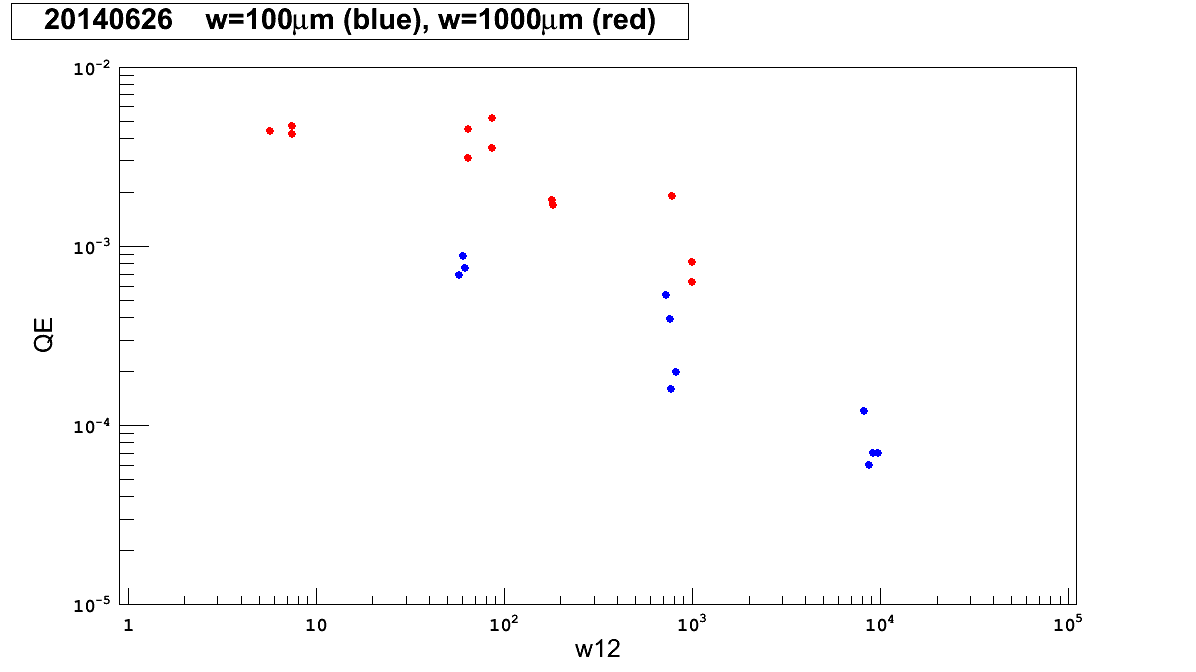
\includegraphics[width=.7\textwidth]{figures/QE_20140626_separate_w.png}
                \caption{\emph{\color{gray}correct this too for real w12 ... or just do I? prolly}, and needs some correction to combine the two regions?}
\label{fig:qe}
\end{figure}

%Another interesting result is the model's inability to explain the low fluorescence efficiency ($\epsilon_{f}$) observed in these peaks.  The number of counts observed is significantly lower than expected from $a_{21} = ?$.  $\epsilon_{f}$, defined in [Ch.2], was measured by the total counts observed in the first frame of exposure divided by its respective $w_{12}$, shown in Fig. \ref{fig:qe}.  This method of measuring $\epsilon_{f}$ becomes less accurate with more optical pumping in the first frame, i.e. with higher $w_{12}$ for a given frame time.  Thus, the trend should be extrapolated toward zero.  Since it seems to be leveling off in the lowest $w_{12}$ values,  the trend suggests a real $\epsilon_{f}$ of about {\color{red}0.5\%}.  The bleaching model was unable to explain this low $\epsilon_{f}$ by additional paths out of the excited state without introducing extreme alterations to existing rates, or by introducing extreme $a_{26}$ and $a_{61}$, in order to dominate $a_{21}$.  A possibility is that the low count rate actually reflects a matrix site population by only about 1\% of deposited Ba\textsuperscript{+} ions.  \emph{\color{gray}I bet $w = 100~\mu m$ is more likely to be the wrong one ... does that one require that more extreme w12 change in modeling (or, the one that still requires a fix after the right P correction has been applied)?}

\section{Candidate Ba\textsuperscript{+} Lines/Blue Excitation}
\label{sec:BaPlus}

Since the fraction of neutralization of Ba\textsuperscript{+} deposited in SXe is not known to be 100\%, in this system and particularly in future tests of grabbing out of LXe, detection of single Ba\textsuperscript{+} in SXe is still of interest.  Preliminary studies of fluorescence from Ba\textsuperscript{+} deposits were performed by blue laser excitation with the C480 dye laser.

\begin{figure} %[H]
        \centering
                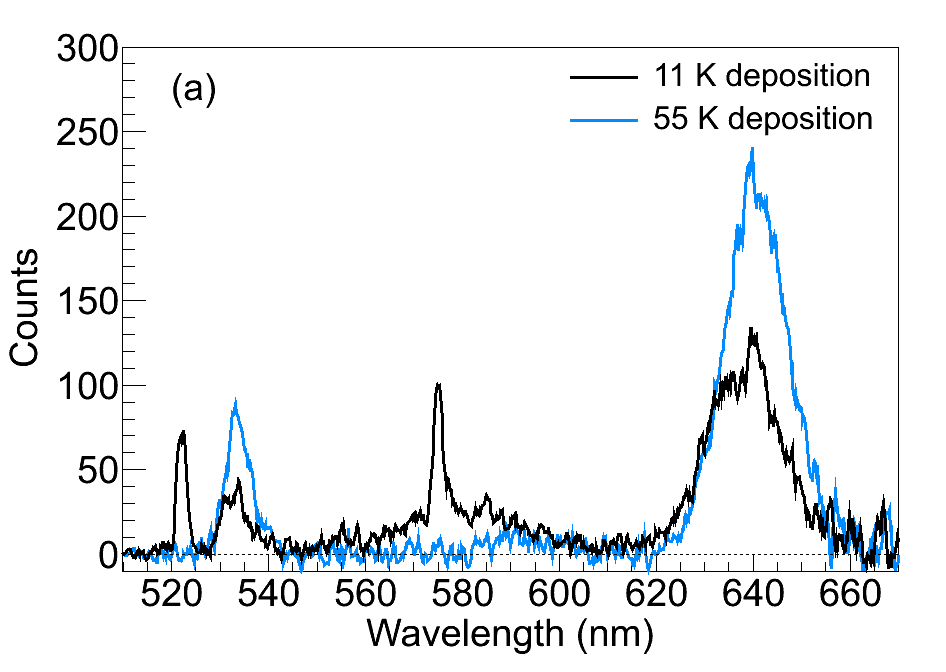
\includegraphics[width=.5\textwidth]{figures/BaHx_a.png}
                ~
                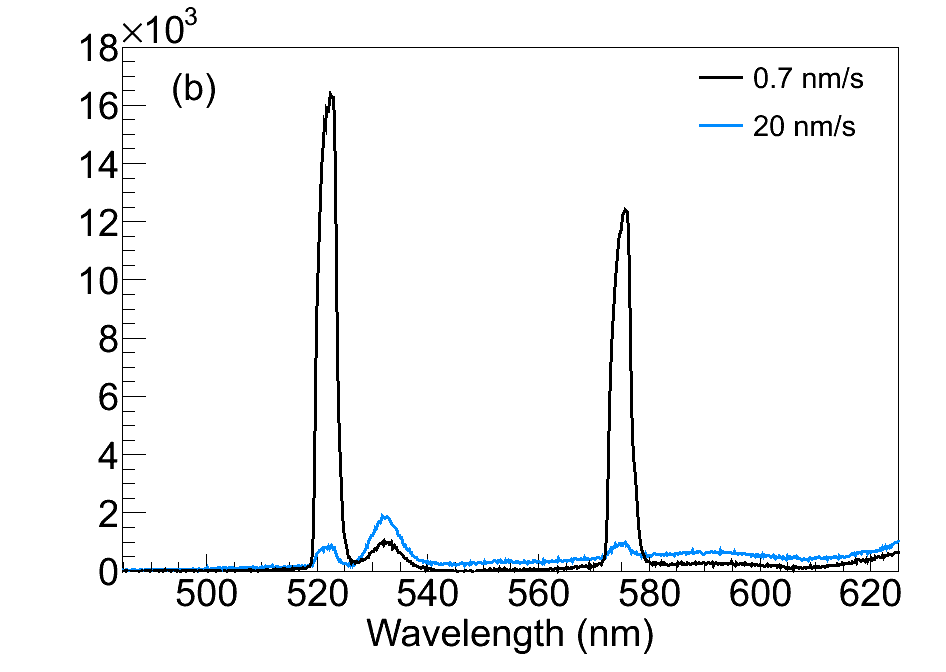
\includegraphics[width=.5\textwidth]{figures/BaHx_b.png}
                \caption{Comparison of Ba\textsuperscript{+} deposits made at (a) 55~K vs. 11~K, and (b) 20~nm/s vs. 0.7~nm/s.\cite{Mong2015}}
\label{fig:BaHx}
\end{figure}

Blue excitation of Ba\textsuperscript{+} in SXe were first explored in the thesis of Shon Cook, wherein a set of sharp emission peaks were observed at 522, 575, 637, 712, and 814~nm, in decreasing amplitude.  These peaks were attributed to emission from different vibrational states of a molecule composed of Ba and one or more H atoms \cite{Shon}.  This attribution is supported by two experiments.  Firstly, a reduction of those peaks is observed in deposits made at 50~K, well above the H$_{2}$ freezing temperature of 12~K, vs. deposits made at 11~K, as shown in Fig. \ref{fig:BaHx}(a).  Secondly, the peaks are much stronger in deposits made with lower leak rates, as shown in Fig. \ref{fig:BaHx}(b), for deposits made at 11~K.  This is explained by a higher concentration of H$_{2}$ impurities in a matrix formed with a lower leak rate.

\begin{figure} %[H]
        \centering
                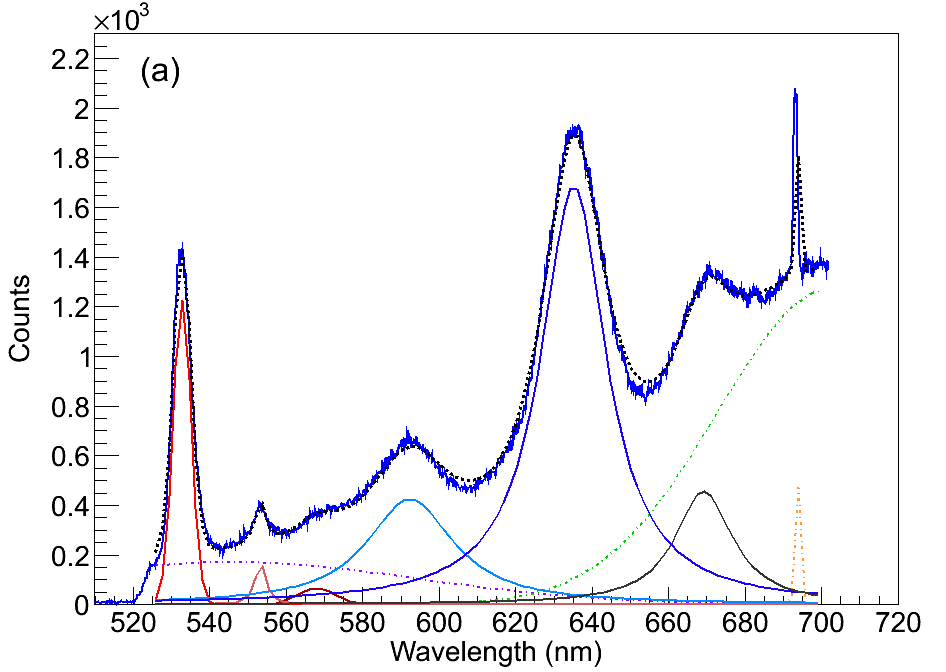
\includegraphics[width=.7\textwidth]{figures/excitspecBlue_a.png}
                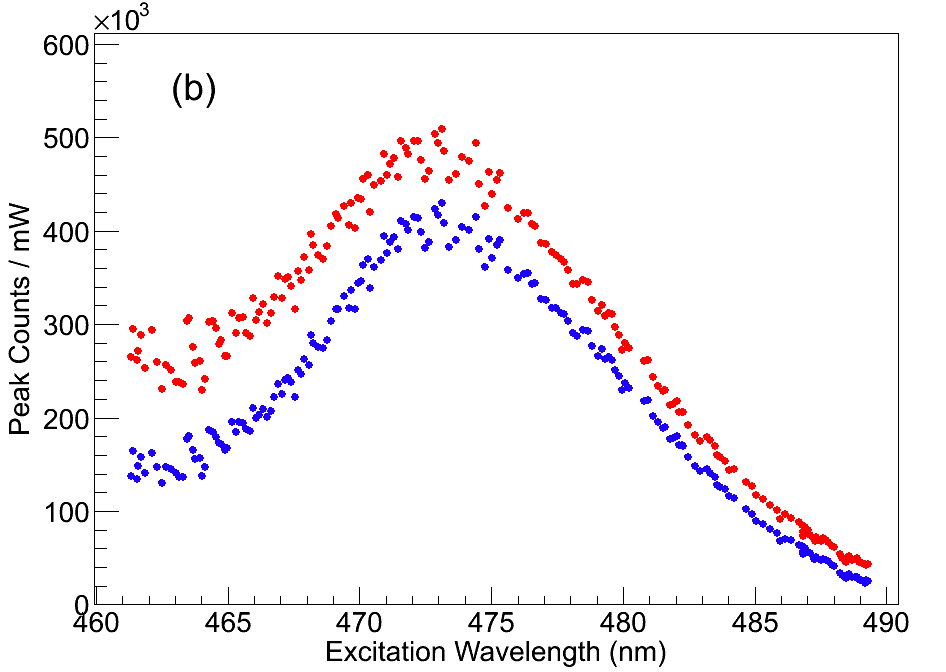
\includegraphics[width=.7\textwidth]{figures/excitspecBlue_b.png}
                \caption{(a) Multiple-component fit to example emission spectrum with 468.2-nm excitation, and (b) excitation spectra for peaks observed through C480 dye range.  In (a), the 532- and 568-nm peaks are fit with Gaussians, and the 553-, 592-, 635- and 669-nm peaks are fit with Lorentzians.}
\label{fig:excitspecBlue}
\end{figure}

In contrast to lower BaH$_{x}$ emission, several other emission peaks become prominent in deposits made at 50$\pm$5~K and observed at 11~K.  A representative spectrum with fits is shown in Fig. \ref{fig:excitspecBlue}(a), and excitation spectra from those fits over the C480 dye range are shown in Fig. \ref{fig:excitspecBlue}(b).  \emph{\color{gray}The broad blue BG ... what does its excitspec look like? is it possible it is the surface BG? ... anyway you need to mention it.}  Of particular interest are the peaks at 532~nm and 635~nm.  These peaks have identical excitation spectra, indicating that they are due to the same excitation transition.  Thus the 532- and 635-nm peaks may be due to relaxation to the ground and metastable D states, respectively, from one of the excited P states of Ba\textsuperscript{+} in SXe.  However, matrix effects would need to be responsible for the higher number of counts observed in the 635nm peak vs. the 532-nm peak, whereas the P $\rightarrow$ S transition is about 4$\times$ more likely than the P $\rightarrow$ D transition in vacuum.  The resemblance between the excitation spectra for the 592- and 669-nm peaks, as well as between the 553- and 568-nm peaks, is also interesting.  

%(a) the much slower bleaching rate than would be observed by optical pumping of Ba\textsuperscript{+} in vacuum, and (b)

%, as well as identical bleaching rates, shown in Fig. [fig 532/635 bleach]